\begin{flushright}
    از حافظه‌های مانا می‌توان به \emph{SSD , memory flash و HDD } اشاره کرد.
    در ادامه قصد داریم نگاهی دقیق تر به \textbf{HDD} بیندازیم.

    ساختار درونی HDD به شکل زیر است.
    \begin{figure}[H]
        \centering
        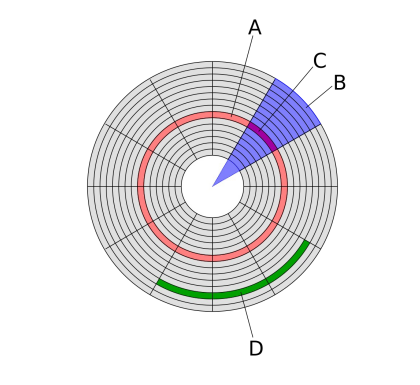
\includegraphics[width=0.7\textwidth]{source/HDD}
        \caption{ساختار درونی دیسک}
        \label{fig:HDD}
    \end{figure}

    \begin{small}
        \begin{enumerate}
            \item[] A شیار: حلقه‌هایی که با کنارهم قرار گرفتن، دیسک را می‌سازند.
            \item[] B قطاع: هندسی قطاعی از دیسک.
            \item[] C قطاع: کوچکترین بلوک حافظه می‌باشد.
            هر \textbf{شیار} می‌تواند شامل تعداد زیادی \textbf{قطاع} باشد.
            \item[] D خوشه: از کنار هم قرار گرفتن چندین \textbf{شیار} ایجاد می‌شود.
        \end{enumerate}
    \end{small}

    \begin{figure}[H]
        \centering
        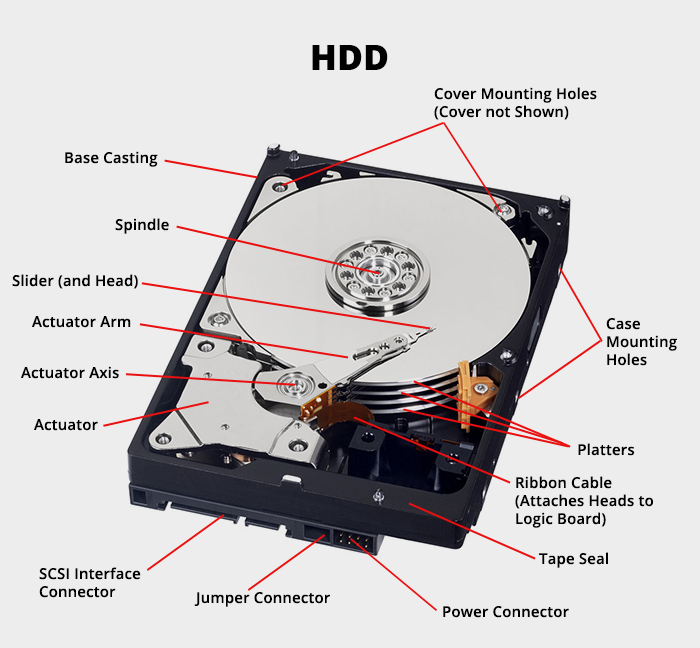
\includegraphics[width=0.7\textwidth]{source/hdd-structure}
        \caption{قسمت‌های مختلف HDD}
        \label{fig:hdd-structure}
    \end{figure}

    بشقاب‌ها
    \footnote{platters}
    توسط چرخاننده
    \footnote{spindle}
    در حال حرکت قرار می‌گیرند.
    برای خواندن از روی بشقاب‌ها، از یک بازو
    \footnote{Actuator arm}
    استفاده می‌شود.
    این بازو می‌تواند به سمت بالا و پایین حرکت کند تا بتواند بر روی شیار‌ها مختلف حرکت کند.

\end{flushright}